\documentclass{article}
\usepackage[utf8]{inputenc}
\usepackage[hidelinks]{hyperref}
\usepackage{amsmath, bm}
\usepackage[noabbrev, capitalise]{cleveref}
\usepackage{amssymb}
\usepackage{graphicx}
\usepackage{float}
\usepackage{subfig}
\usepackage{booktabs}
\usepackage[parfill]{parskip}

\usepackage[sorting=none]{biblatex}
\addbibresource{report_2.bib}

\usepackage{titling}
\setlength{\droptitle}{-3cm}

\title{COMP6247 Lab 2: Kalman Filter}
\author{Wei Chien Teoh (Eugene)\\\bigskip \href{mailto:wct1c16@soton.ac.uk}{wct1c16@soton.ac.uk}}
\date{4 March 2021}

\begin{document}

\maketitle

\section{Introduction}

This report presents the findings and results for Lab 2 of COMP6247 of University of Southampton \cite{lab2}. The code implementation is stored in a Github repository \cite{github}.

First, a random excitation signal is generated using Numpy sampled from a normal distribution, $X \sim \mathcal{N}(0, 1)$. The excitation signal is then transformed into a second order autoregressive (AR) time series.

Two AR series are generated. One with constant parameters, $\mathbf{a} = (1.2, -0.4)^T$. Another is with time-varying parameters defined in \cref{eq:non-stationary_ar}. The signal plots will not be shown as it is identical to the ones in \cite{lab2}.

\begin{subequations}
    \label{eq:non-stationary_ar}
    \begin{align}
        a_0(t) &= \frac{1}{10} \cos(\frac{2 \pi t}{400}) + 1.2 \\
        a_1(t) &= \frac{1}{10} \sin(\frac{\pi t}{400}) - 0.4
    \end{align} 
\end{subequations}

% \begin{figure}[h!]
%     \centering
%     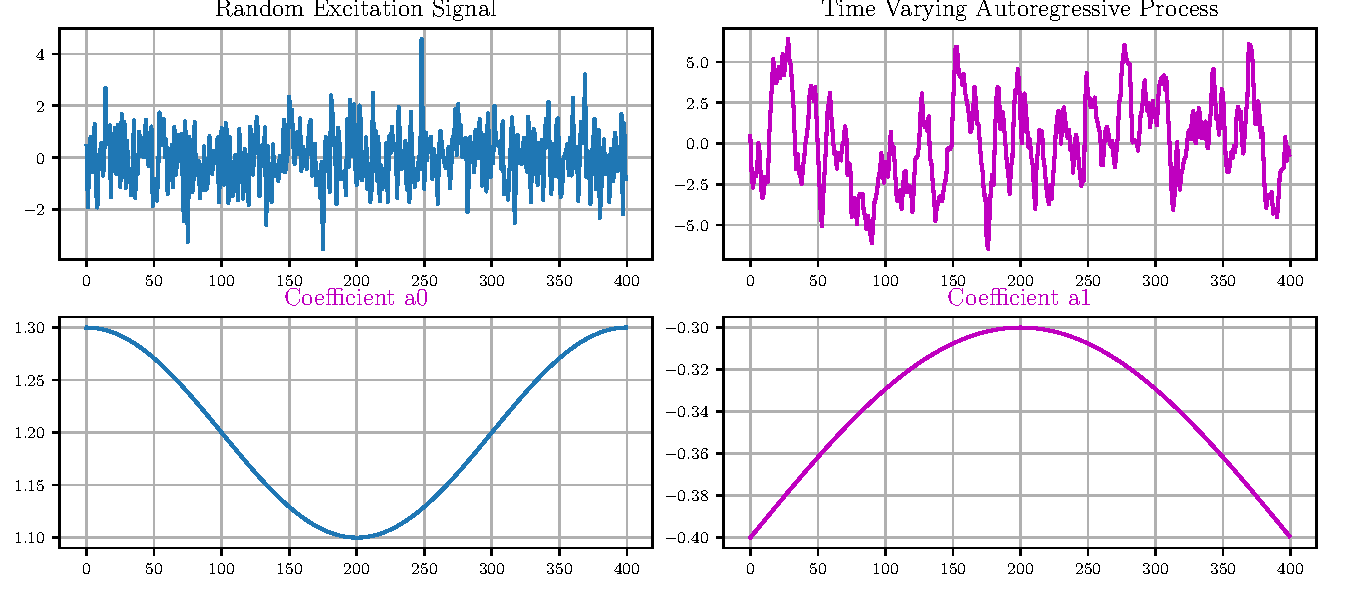
\includegraphics[width=\textwidth]{Figures/non-stationary_ar.pdf} 
%     \caption{(Top left) Random excitation signal. (Top right) Second order autoregressive process of excitation signal with time-varying coefficients. (Bottom left) Coefficient $a_0$. (Bottom right) Coefficient $a_1$.}
%     \label{fig:non-stationary_ar}
% \end{figure}

A Kalman Filter is used for state estimation of the parameters of the both the stationary and time-varying AR process. The effects of initial conditions, process noise covariance and measurement noise variance on the convergence on the state estimation are explored.


\section{Effects of Initial Conditions}

In this section, the effects of initial conditions $\bm{\theta}(0|0)$ and $\bm{P}(0|0)$ on the convergence of the parameter estimation is explored. Throughout the experiment in this section, the process noise covariance $\bm{Q}$ and measurement noise variance $R$ are set to $0.01I$ and the variance of the AR process, respectively. Both stationary and non-stationary plots have similar effects when initial conditions are changed, hence only the stationary plots will be shown in this section.

\subsection{Initial State} \label{sec:initial_state}

Five different initial values of initial state $\bm{\theta}(0|0)$ will be explored. The initial value of the posteriori estimate covariance $\bm{P}(0|0)$ is set to $0.001I$. \cref{fig:initial} shows the convergence of five different initial state values, namely:
\begin{enumerate}
    \item Random values generated from Numpy, $\bm{\theta}(0|0) \sim \mathcal{N}(0, 1)$;
    \item $(0, 0)^T$;
    \item $(100, 100)^T$;
    \item $(1.2, -0.4)^T$;
    \item $(-100, -100)^T$;
\end{enumerate}

It is shown that all five different initial values of $\bm{\theta}(0|0)$ eventually converges to the same values after certain number of iterations. However, initialising the values closer to the true values allow for a faster convergence. Hence, it can be concluded that $\bm{\theta}(0|0)$ does not affect the convergence of the parameter estimation, but tuning it will increase the convergence speed.

\begin{figure}[h!]
    % \subfloat[Stationary AR]{\label{fig:initial_stationary}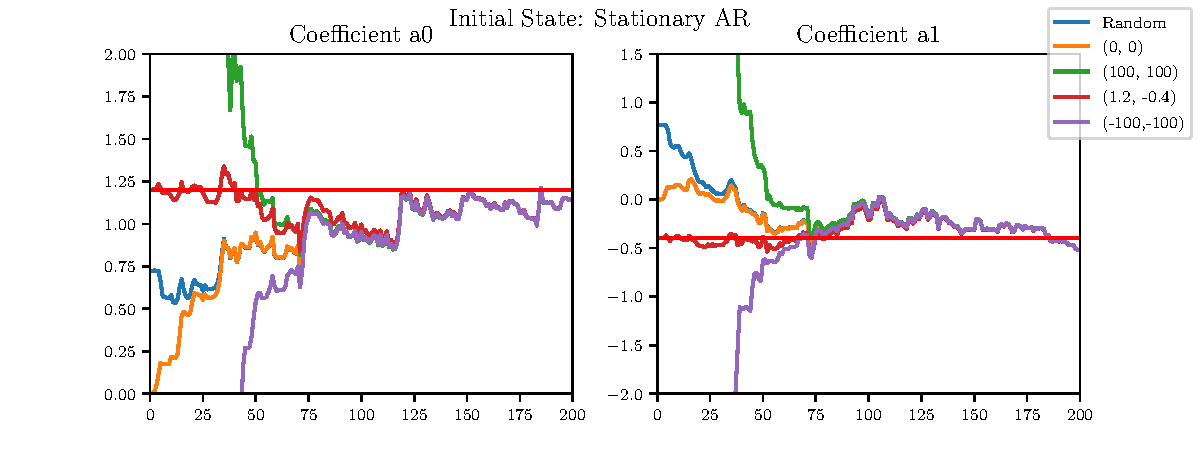
\includegraphics[width=\textwidth]{Figures/initial_stationary.pdf}}\\
    % \subfloat[Non-stationary AR]{\label{fig:initial_non-stationary}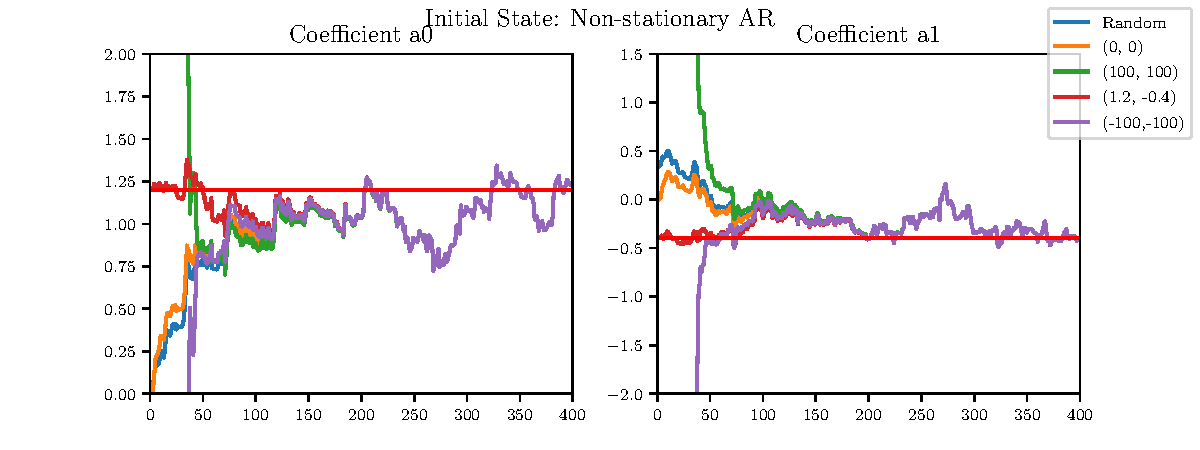
\includegraphics[width=\textwidth]{Figures/initial_non-stationary.pdf}}
    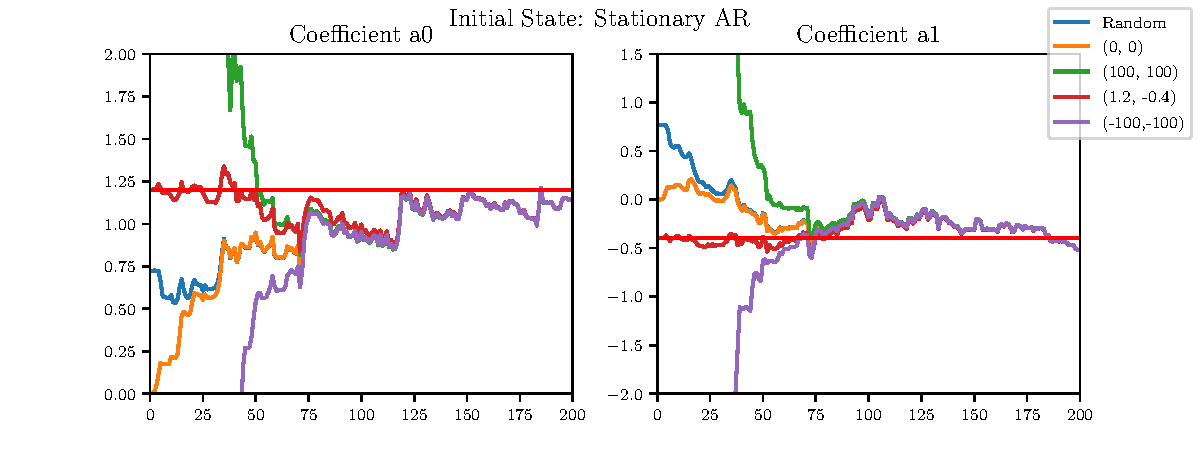
\includegraphics[width=\textwidth]{Figures/initial_stationary.pdf}
    \caption{Stationary AR parameter estimation with different initial states.}
    \label{fig:initial}
\end{figure}

\subsection{Initial Parameter Covariance}

Five different initial values of initial state covariance $\bm{P}(0|0)$ will be explored. The initial value of the posteriori state estimate $\bm{\theta}(0|0)$ is set to $\bm{\theta}(0|0) \sim \mathcal{N}(0, 1)$. \cref{fig:initial_cov_stationary} shows the convergence of five different initial covariance values, namely:
\begin{enumerate}
    \item $0.001I$;
    \item $Var(ex)I$, the variance of the excitation signal;
    \item $1000I$;
    \item $0I$;
    \item $I$;
\end{enumerate}


\begin{figure}[h!]
    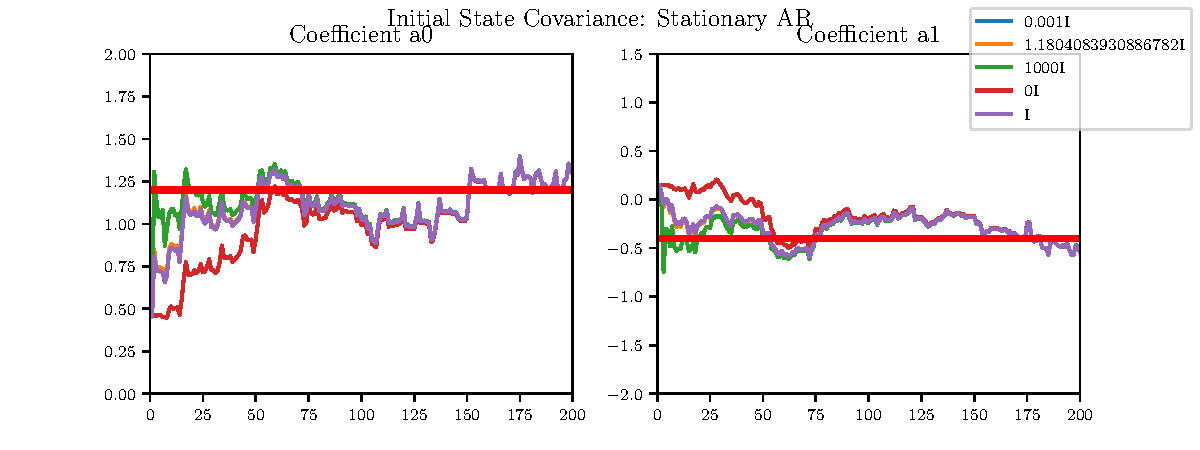
\includegraphics[width=\textwidth]{Figures/initial_cov_stationary.pdf}
    \caption{Stationary AR parameter estimation with different initial state covariances.}
    \label{fig:initial_cov_stationary}
\end{figure}

Similar to \cref{sec:initial_state}, all five different initial values of $\bm{P}(0|0)$ eventually converges to the same values after certain number of iterations. $\bm{P}(0|0)$ signifies the estimation confidence of the initial parameter estimate $\bm{\theta}(0|0)$. Setting $\bm{P}(0|0)$ to a large value allows more fluctuations in the initial iterations but faster convergence, as shown in the green line in \cref{fig:initial_cov_stationary}.

\section{Effects of Process Noise}

\cref{fig:process} shows the convergence of parameters with different values of process noise covariance $Q$. For this section's experiment, the following initial values and parameters are set:
\begin{itemize}
    \item $\bm{\theta}(0|0) \sim \mathcal{N}(0, 1)$;
    \item $\bm{P}(0|0) = 100I$;
    \item $R = Var(Observation)$;
\end{itemize}

For the stationary AR process, three values of $Q$ are chosen, namely: $0I$, $0.01I$, $0.5I$. For the non-stationary AR process, only two values of $Q$ are chosen, namely: $0I$ and $0.01I$. From \cref{fig:process}, we can see that for both stationary and non-stationary AR processes, increasing the value of $Q$ does not contribute to the convergence. Rather, it introduces more variance and fluctuations of the convergence. Setting $Q$ to $0I$ provides the most stable and better convergence. This is reasonable as no noise was introduced when the AR time series is generated from the excitation signal.

For non-stationary AR process, with $Q = 0I$, \cref{fig:process_non-stationary} show that the estimation is able to capture the time-varying parameter. However, there is a small lag with the parameter estimation, thus being insensitive to time-varying parameters.


\begin{figure}[h!]
    % 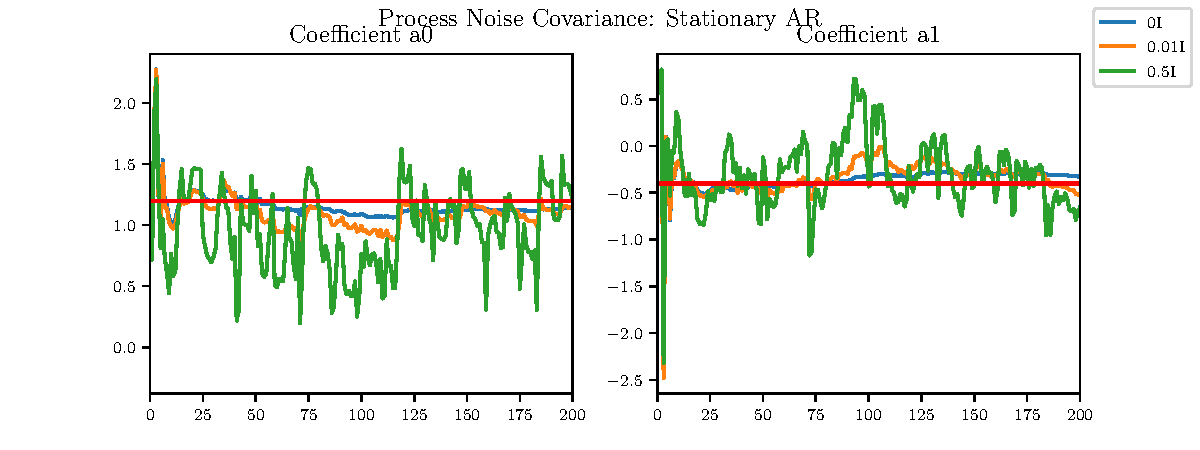
\includegraphics[width=\textwidth]{Figures/process_noise.pdf}
    \subfloat[Stationary AR]{\label{fig:process_stationary}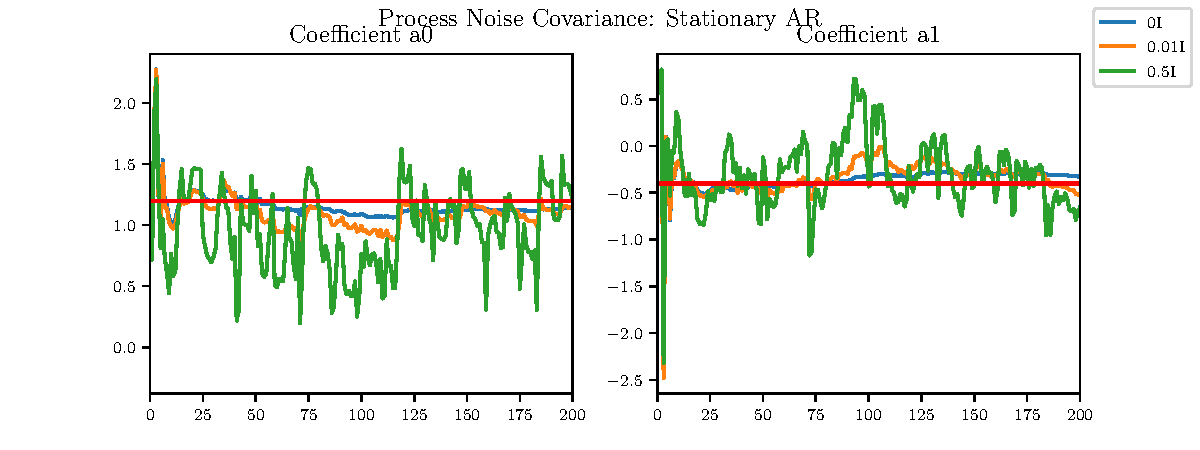
\includegraphics[width=\textwidth]{Figures/process_noise.pdf}} \\
    \subfloat[Non-statinoary AR]{\label{fig:process_non-stationary}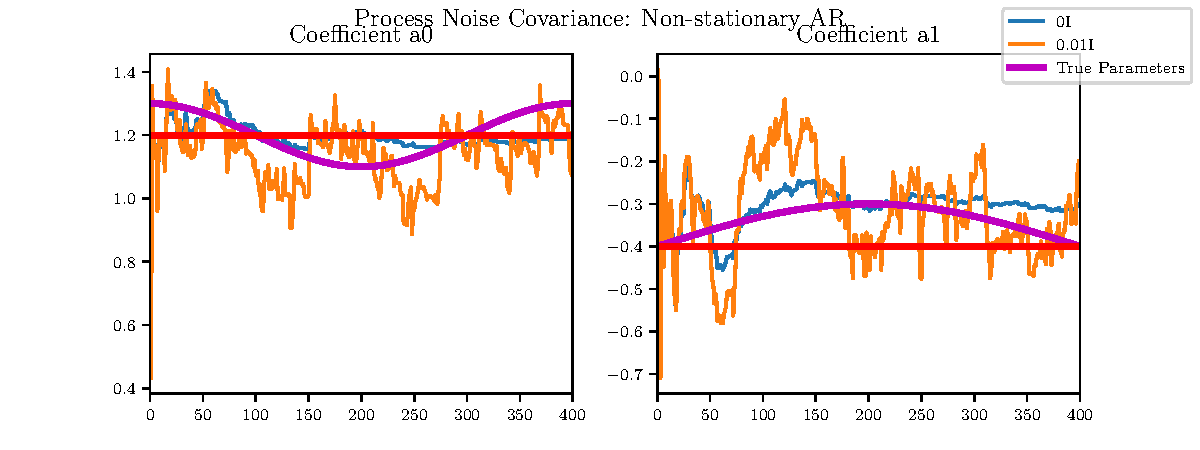
\includegraphics[width=\textwidth]{Figures/process_noise_non-stationary.pdf}}
    \caption{AR parameter estimation with different process noise covariance Q.}
    \label{fig:process}
\end{figure}

\section{Effects of Observation Noise}

\cref{fig:observation} shows the convergence of parameters with different values of observation noise variance $R$. For this section's experiment, the following initial values and parameters are set:
\begin{itemize}
    \item $\bm{\theta}(0|0) \sim \mathcal{N}(0, 1)$;
    \item $\bm{P}(0|0) = 100I$;
    \item $\bm{Q} = 0.001I$
\end{itemize}

For both stationary and non-stationary AR process, three parameters are set, namely: $0.01$, $Var(Observation)$, $10000$, where $Observation$ is the AR process. From \cref{fig:observation}, it is shown that smaller values enables faster convergence. However, for values that are too small, in this case $R < 0.1$, more fluctuation and variance of the parameter estimation is introduced. For larger values, there are less fluctuations and more stable convergence at the expense of slower convergence.

In many applications, $R$ is set the the variance of the observation if it is known \cite[p.~265]{labbe2020}. \cref{fig:observation} shows that by using the variance of the observation, it is able to provide reasonable convergence speed with less noise. However, $R$ is a parameter to be further tuned from prior knowledge of the problem. 

\begin{figure}[h!]
    \subfloat[Stationary AR]{\label{fig:observation_stationary}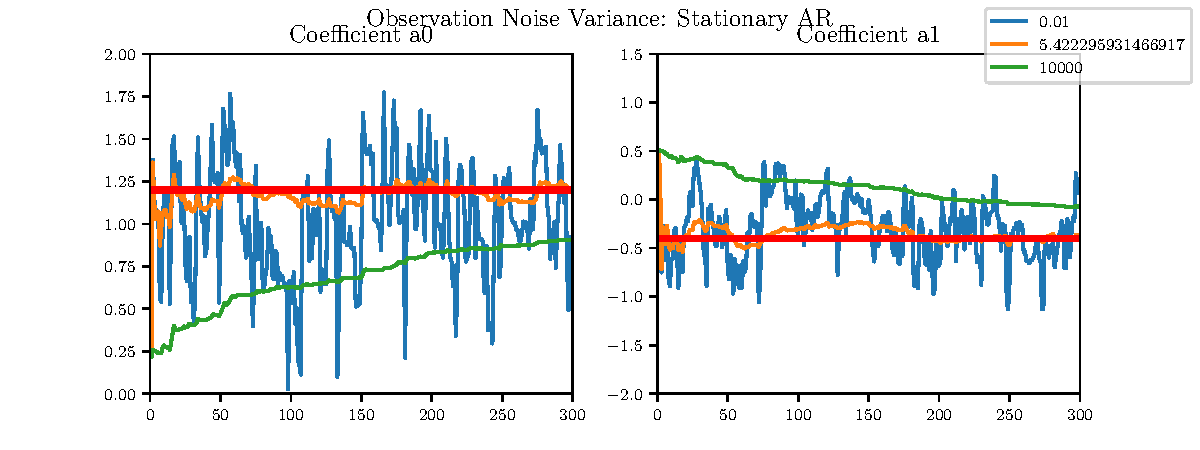
\includegraphics[width=\textwidth]{Figures/observation_stationary.pdf}} \\
    \subfloat[Non-stationary AR]{\label{fig:observation_non-stationary}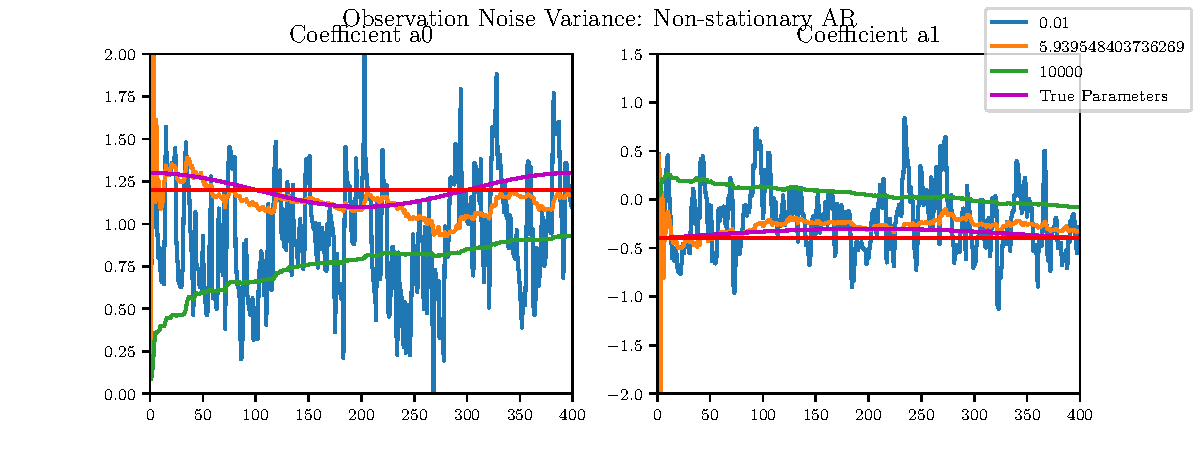
\includegraphics[width=\textwidth]{Figures/observation_non-stationary.pdf}}
    \caption{AR parameter estimation with different observation noise variance R.}
    \label{fig:observation}
\end{figure}





\printbibliography

\end{document}